 \section{Methodology}
\label{sec:Method}
Prior to proposing more specific guidelines for developing a tactic search engine, we conducted an extensive study of architectural decisions in performance centric and dependable complex system.

\subsection{Goals}
 We believe that the current literature lacks insight into tactic's implementation. Revealing the low-level and non-abstract issues in coding architectural tactics can help shape the foundations of a tactic search engine. 
 
 \subsection{Research Question}
Our study was concerned about the following research high-level research question:
RQ: What are the inherent characteristics of tactics implementations?

\subsection{Project Selection}
The following process was used to select a set of open source projects for this study.

\begin{itemize}
\item \textit{Selection through Code Search:} The source code search engine \textit{Koders} was used to search for the projects which have implemented a set of predefined architectural tactics. The search query for each tactic was composed from keywords used in  the libraries that architect has previously used to implement the tactics. the results have been peer reviewed to ensure that each project has implemented the architectural tactic.
\item \textit{Selection by Meta-Data:} Project-related documents, such as design documents, online forums, etc. were searched for references and pointers to architectural tactics. This search was followed with a detailed source code search to ensure each identified project has the tactics implemented as well.
\end{itemize}
We have identified 40 open source projects using this process. The projects are elicited from different application domains, with diverse size, and developed using different programming languages. These dataset included projects such as Chromium, Apache Hadoop, Ofbiz and Hive which are comparable to industrial applications.

\subsection{Study: Learning from the Trenches}
For each of the studied projects we identified architecturally significant requirements, architectural tactics used to address them and source files used to implement tactics.
For each of identified tactic, a peer-code review has been conducted to extract code snippets implementing the tactics. This was then followed by a manual reverse engineering process where our team members have utilized Enterprise Architect reverse engineering features to \textit{draw a class diagram for each instance of the tactic}. In this study, two code reviewers with software architecture background were asked to document their observations of tactics implementations and formulates the challenges that impacts the development of a tactic search engine. 
The following section presents the results of this study.
\section{Qualitative Study}
\label{sec:SeenUnSeen}
As a result of this study we observed five issues related to our research questions that can also significantly influence development of any practical tactic search engine:

\subsection{No Single Solution}
There is no single way to address a quality requirements and also no single way to implement an architectural tactic. From one system to another system a tactic can be implemented entirely differently, this divergence is due to the differences in the context and constraints of each projects.

For example, we reviewed the implementation of \emph{heartbeat} tactic for reliability concerns in 20 different software systems. We observed the heartbeat tactic being implemented using (i) direct communication between the emitter and receiver roles found in~\emph{(Chat3 and Smartfrog systems)}, (ii) the observer pattern in which the receiver is registered as a listener to the emitter found in the \emph{Amalgam system}, (iii) the decorator pattern in which the heartbeat functionality was added as a wrapper to a core service found in~\emph{(Rossume} and~\emph{jworkosgi systems)}, and finally (iv) numerous proprietary implementations which did not follow any documented design notion.

\textit{Therefore a tactic-search engine can not primarily rely on structural dependencies as a means of learning the best tactic implementation.}

\begin{figure}[!htb]
\centering

\subfigure[HeartBeat with configuration files]{
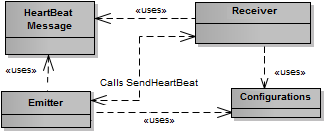
\includegraphics[width=.4\textwidth]{img/HB1.png}
\label{fig:HB1}
}

\subfigure[Observer design pattern to implement the tactic]{
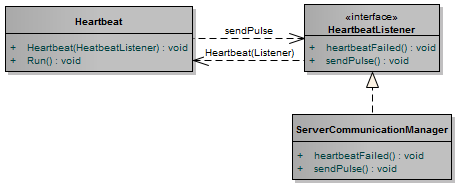
\includegraphics[scale=0.45]{img/HB2.png}
\label{fig:HB2}
}
\subfigure[Decorator design pattern to implement the tactic]{
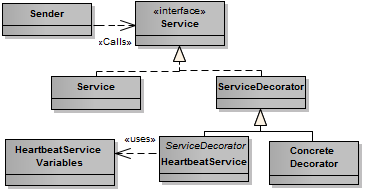
\includegraphics[width=.45\textwidth]{img/HB3.png}
\label{fig:HB3}
}
\label{fig:HBall}
\caption[Heartbeat tactic in different systems]{Hadoop : \subref{fig:HB1}Hadoop, Chat3, smartfrog \subref{fig:HB2}Amalgam System \subref{fig:HB3}Thera, JSRB, Rossume Systems}
\end{figure}

\begin{figure}[tbph]
\centering
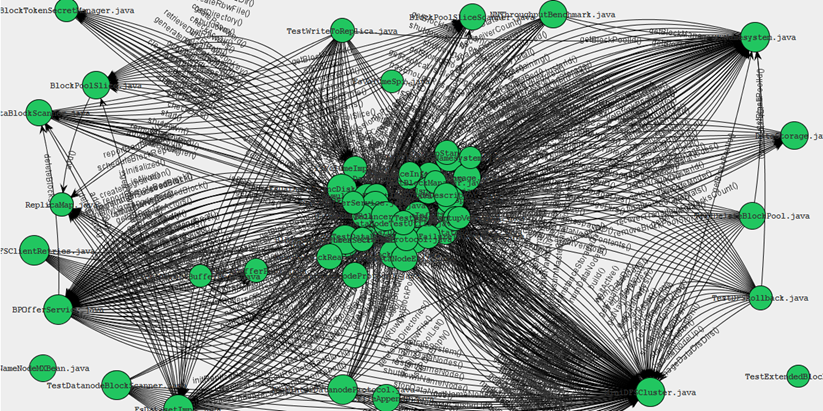
\includegraphics[width=0.99\linewidth]{./img/Pooling}
\caption{Resource Pooling Tactic Implemented in Apache Hadoop Project}
\label{fig:Pooling}
\end{figure}


\subsection{Structure Is Not a Key, But Impacts Code Quality}
Unlike design patterns, which tend to be described in terms of classes and their associations, tactics are described in terms of roles and interactions~\cite{bass:arch12}. This means a tactic is not dependent upon a specific {\em structural} format. While a single tactic might be implemented using a variety of design notions or proprietary designs, the structural properties of tactical files can have significant on the quality of the tactic. Flaws such as cyclic dependencies, improper inheritance, unstable interfaces, and modularity violations are strongly correlated to increased bug rates and increased costs of maintaining the software.

Figure \ref{fig:Pooling} visualizes the\textit{ resource pooling} tactic in Apache Hadoop project. Nodes in this graph represent the source file, and the edges are method calls between the source files. We observed several tactic implementations that did not exposed a well organized structure, typical they formed a full graph with several cyclic dependencies between each pair of files. 

\textit{A tactic-search engine should take into account the internal quality of recommended code to avoid suggesting codes with design and structural flaws.}


\subsection{Tactical Clones, Right Level of
\\Reuse-Granularity}
While the implementation of tactics are different from one system to another system, the \textit{intrinsic characteristics of tactics are maintained across different projects}. We call these as \emph{architectural or tactical clones}. Based on our observation, tactical clones are the minimum reusable tactical features.
In our code review process, we found that even for a simple tactic like heartbeat the implementation would result in a large number of interrelated files, each playing different roles such as \textit{heartbeat emitter}, \textit{heartbeat receiver}, \textit{configuration files} to set heartbeat intervals and other parameters,\textit{ supporting classes and interfaces} to implement each  tactical roles. More complex tactics, specially the cross-cutting ones can easily impact hundreds of source files. Therefore recommending code snippets for those tactics would create a large search space for the developers with lesser degree of reusability. 

\textit{The lack of structure, and a concrete micro-level design which can be recovered across multiple projects indicates that method level clones are the right level of granularity. } In the next section of this paper we provide examples of such tactical clones.

\subsection{Tactics Are Misused, Degraded or Implemented Incorrectly.} Open source repositories contain several cases where architectural tactics have been adopted by the developers without fully understanding the driving forces and variability points \cite{FSE2012} associated with each tactic and consequences of implementing the tactic. The Heartbleed issue is a good example of such misuse. Heartbeat functionality in OpenSSL is an optional feature, while many developers could have easily disabled it in configuration files they fully ignored that. Furthermore, the implementation of heartbeat functionality did not followed solid software engineering practices.

In our analysis of bug reports in tactical fragments of the Hadoop project, we found that if a tactical file had a bug, then 89\% of these issues were due to issues such as unhandled exceptions, type mismatches, or missing values in a configuration file.
11\% of reports where due to wrong implementation. These bugs involved misconceptions in the use of the tactic, so that the tactic failed to adequately accomplish its architectural task.  These kinds of bugs caused the system to crash under certain circumstances. For example, in one case a replication decision with a complex synchronization mechanism was misunderstood for different types of replica failure. Another example was a scheduling tactic which resulted in deadlock problem. This investigation shows that systems are exposed to new risks during implementation of the tactical decisions. 

\textit{A practical tactic search engine needs to take into account tactical code qualities, the context in which the tactics are adopted and the historical bug fixes and refactoring activities on candidate clone for recommendation.} 


\subsection{Object Oriented Metrics Are Not Indicator of Tactical Code Quality}
We performed a detained investigation of bug fixes in two of the systems included in our study. Our initial analysis of Chidamber and Kemerer's OO metrics~\cite{491650} and tactical code snippets in Apache Hadoop and OfBiz systems indicates that tactical code snippets tend to relatively a have higher code complexity compared to non-tactical code snippets~\cite{MSRBuble}. For example implementing \textit{thread pooling} requires devising solutions for \textit{thread safe} problem which will results in a more complex implementation. Therefore OO metrics such as \emph{WMC (Weighted Methods per Class)} or~\emph{CBO (Coupling Between Object classes)} can not solely be a good indicator of an improved tactical code snippet. 

\textit{A good tactic search engine must take into account novel code metrics to filter potentially complex code samples which are difficult to comprehend and modify.}